\begin{figure}[h!]
	\centering
	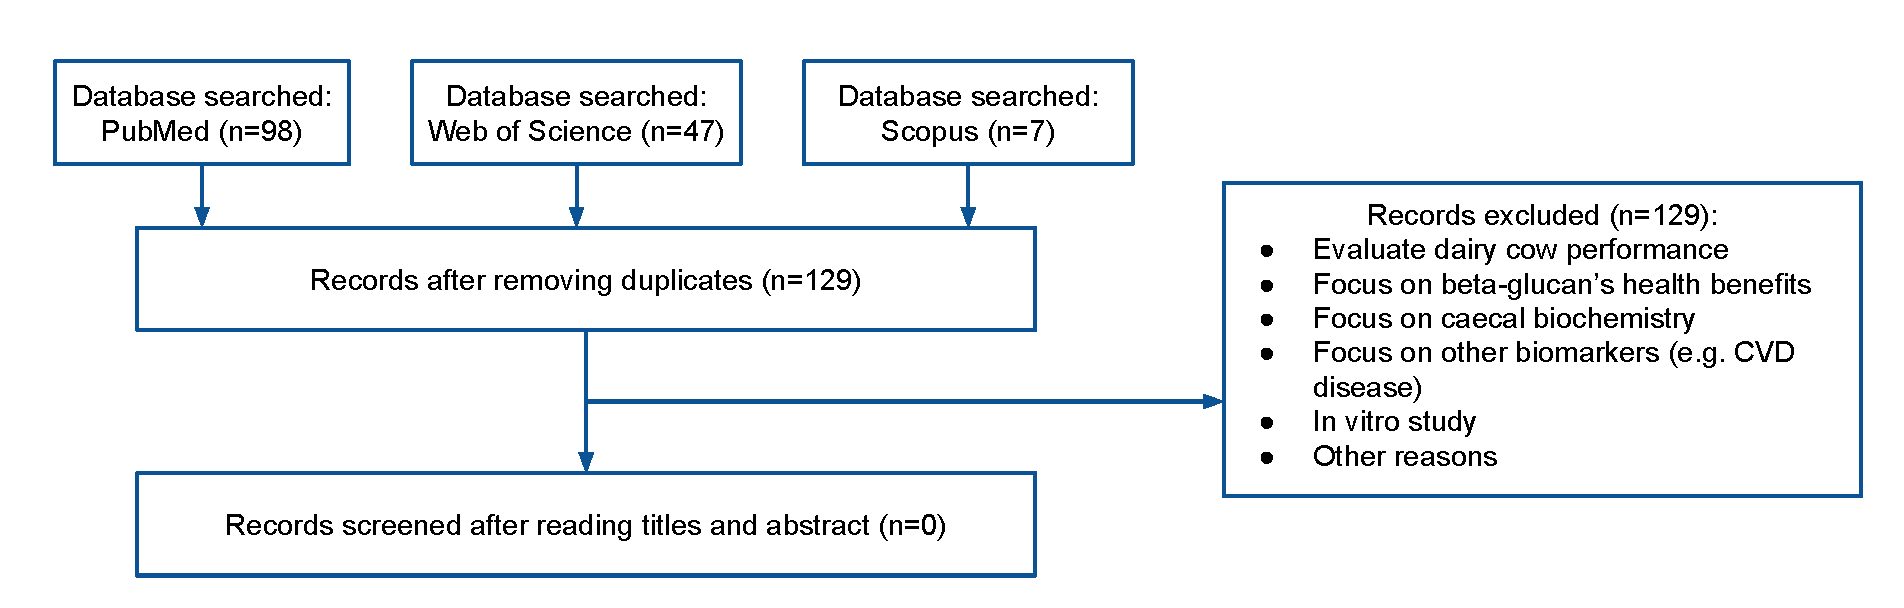
\includegraphics[width=\linewidth]{picture/barley_biomarker_review}
	\caption{Flow chart of literature searching and screening for articles of barley intake biomarkers}
	\label{fig:barleybiomarkerreview}
\end{figure}



%%%%
\begin{landscape}
	\begin{table}[h!]
		\scalebox{0.7}{
			\begin{tabular}{|c|c|c|c|c|c|c|}
				%header
				\hline 
				\makecell{Dietary\\factor} &  \makecell{No.\\subjects} &\makecell{Study\\design} & \makecell{Sample\\type}  & \makecell{Analytical\\method} & \makecell{Candidate\\biomarker(s)} & Reference \\ 
				\hline
				%1st entry - betaine
				\makecell{Wheat bran,\\Wheat aleurone} & 14+13 & \makecell{randomized,\\ cross-over,\\ intervention} & \makecell{plasma}  & \makecell{LC-MS/MS\\ (Microbiology assay\\for folate)} & \makecell{betaine\\choline\\folate\\dimethylglycine (DMG)} & \cite{ISI:000350230300006} \\ 
				\hline
				
				%2nd entry - PREDIMED
				\makecell{None-bread,\\White bread,\\WG bread} & 155 & observation\footnote{dietary exposure measured from FFQ} & \makecell{\makecell{urine}}  & HPLC-qTOF-MS & Benzoxazinoid-related metabolites (HHPAA, HBOA glycoside) ARs-related metabolites(DHPPA glucuronide, DHPPTA sulphate), microbial-derived metabolites () & \cite{ISI:000348343300015} \\ 
				\hline
				
				%\hline 
				
		\end{tabular}}
		\caption{Reported markers distinguishing WG wheat intake, but NOT specific}
		\label{table:wheat_notspecific}
	\end{table}
\end{landscape}
